\documentclass[12pt]{article}

\usepackage[top=1in,bottom=1in,left=1in,right=1in]{geometry}
\usepackage{amsmath,amssymb,mathtools}
\usepackage{xcolor}
\usepackage{graphicx}
\usepackage{hyperref}

\hypersetup{
    pdfauthor={},
    pdftitle={MATH 1075 - Lesson 6.1 Recitation}
}

\begin{document}

\vspace*{0.5in}

\begin{center}
    {\LARGE MATH 1075 - Section 7.5 Worksheet}

    \vspace{2em}

    {\large 09/22/2026}
\end{center}

\begin{figure}[htbp]
    \centering
    % Replace "my_image" with your actual file name (without extension)
    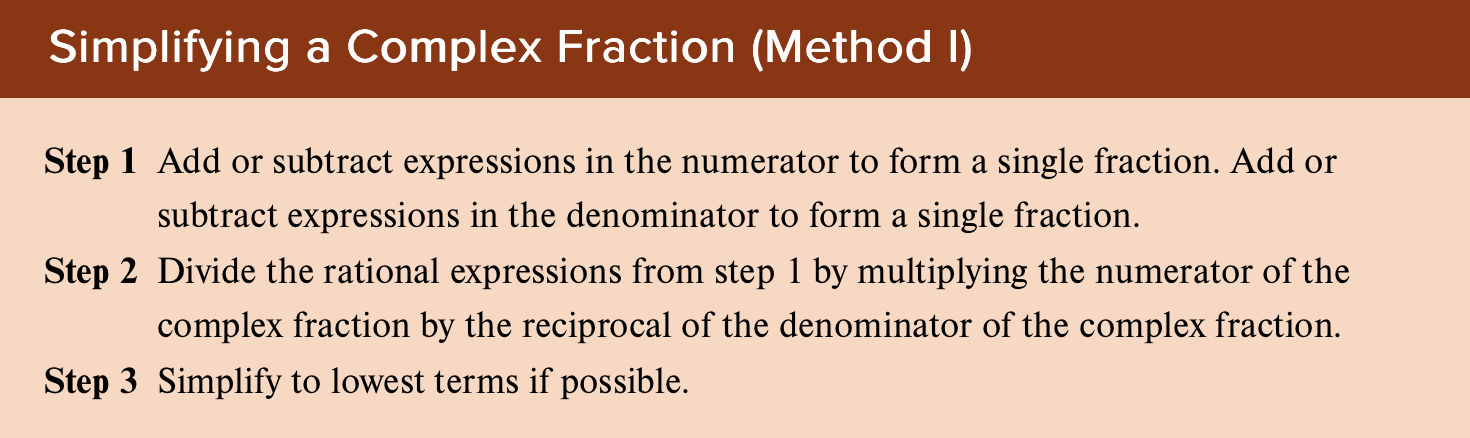
\includegraphics[width=0.9\linewidth]{Method 1.png} 
    \label{fig:my_figure}
\end{figure}
Simplify following complex fractions using method 1
\vspace{1.5em}

1. $\frac{\frac{a^{2}}{2a-3} }{\frac{5a}{8a-12} }  $

\vspace{4.5em}

2. $\frac{\frac{12x^{2}}{5y} }{\frac{8x^{6}}{9y^{2}} }   $

\vspace{4.5em}

3. $\frac{\frac{8}{9}-\frac{1}{3}  }{\frac{7}{6}+\frac{1}{9}  }   $

\vspace{4.5em}

4. $\frac{\frac{1}{b}+1 }{\frac{1}{b} }  $

\vspace{4.5em}

5. $\frac{2+\frac{1}{x} }{4+\frac{1}{x} } $

\newpage

\begin{figure}[htbp]
    \centering
    % Replace "my_image" with your actual file name (without extension)
    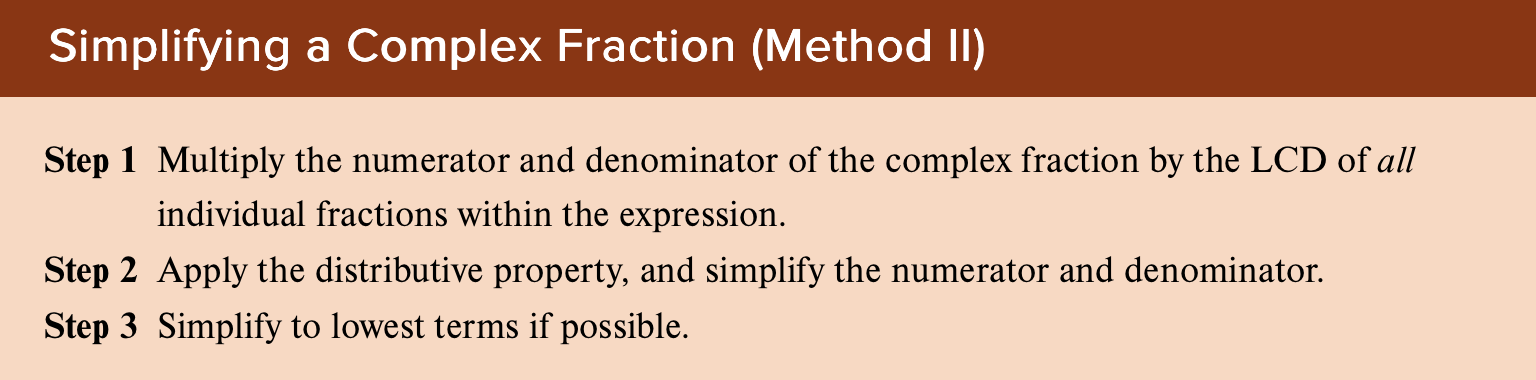
\includegraphics[width=1\linewidth]{Method 2.png} 
\end{figure}
\noindent Simplify following complex fractions using method 2
\vspace{1.5em}


1. $\frac{2+\frac{1}{x} }{4+\frac{1}{x} } $

\vspace{4.5em}

2. $\frac{\frac{8}{9}-\frac{1}{3}  }{\frac{7}{6}+\frac{1}{9}  }   $

\vspace{4.5em}

3. $\frac{1-\frac{9}{p^2} }{1-\frac{1}{p}-\frac{6}{p^2}  } $

\vspace{4.5em}

4. $\frac{\frac{9}{4m}+\frac{9}{2m^{2}}  }{\frac{3}{2}+\frac{3}{m}  } $



\end{document}
